\section{Data and Results}

Our dataset is a combination of cryptocurrencies and classical assets (commodities, exchange rates and stocks), covering the time period 10/20/2014 - 10/16/2018 (1006 trading days), for $n=544$ assets (see \hyperref[table:data]{Table 2}).
The reason for choosing this time-span for the analysis is that before 2015 the liquidity in the cryptocurrencies market had been relatively low, the total market capitalization being less than 16 billion US dollars \citep{Feng.2018}.

\begin{table}[H]
\centering
\small{
	\caption{: Dataset}
	\label{table:data}
\begin{tabular}{l S[table-format=-1.2,table-figures-uncertainty=1] l}\hline\hline
\multicolumn{1}{l}{\bfseries Type of Asset}& \multicolumn{1}{c}{\bfseries Number of Assets}& \multicolumn{1}{c}{\bfseries Source}\\ \hline
Cryptocurrencies&14&Coinmarketcap\\
Stocks&497&Bloomberg\\
Exchange rates&13&Bloomberg\\
Commodities&20&Bloomberg\\ \hline\hline
\end{tabular}}
\end{table}

The first component of the dataset contains a representative sample of cryptocurrencies; the cryptocurrencies selected to be part of this analysis are the components of the CRIX Index \citep{Hardle.2018}, sourced from \url{https://coinmarketcap.com/}, for the time interval 10/20/2014 - 10/16/2018. \href{http://thecrix.de/}{The CRyptocurrency IndeX} is a benchmark for the cryptocurrencies market, being realtime computed by the Ladislaus von Bortkiewicz Chair of Statistics at Humboldt University Berlin, Germany. The 15 components of the CRIX index (see the \hyperref[appendix:a]{Appendix A}) account for 90\% of the total cryptocurrencies market capitalization, as seen in \hyperref[fig:figure_1]{Figure 1}. In our analysis, the USDT cryptocurrency was discarded due to the fact that it is an atypical digital currency, having very little variation around the reference value of 1 USD.
\begin{figure}[H]
	\centering
	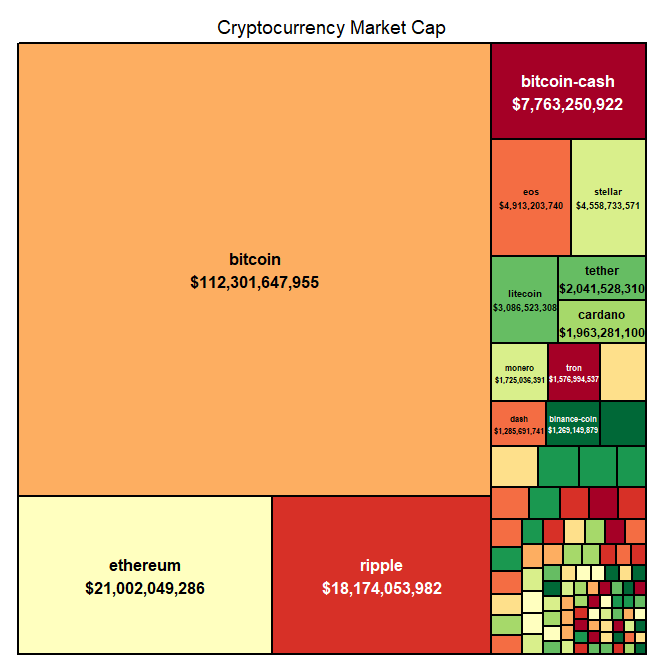
\includegraphics[width=0.5\textwidth]{Fig/figure_1.png}
	\caption{Cryptocurrencies market capitalization (USD) at 10/19/2018\href{https://github.com/QuantLet/Genus_proximum_cryptos/tree/master/Mkt_Cryptos}{. Mkt\_cryptos.}}
	\label {fig:figure_1}
\end{figure}

The second component of the dataset contains a sample of the most traded commodities indexes, according to Bloomberg (see the \hyperref[appendix:a]{Appendix A}).\\
\indent The third component of the dataset contains a sample of the most liquid exchange rates, according to Bloomberg (see the \hyperref[appendix:a]{Appendix A}).\\
\indent The fourth component of the dataset contains the constituents of the S\&P500 Index, recorded at October 19th 2018. The number of constituents of S\&P500 Index is 505, however in our dataset only 497 of them are listed, i.e. those stock with valid data for the entire time period analysed (the complete list of the stocks included in the analysis can be found in the \hyperref[appendix:a]{Appendix A}).

\subsection{Factor Analysis}

Factor analysis is a classical method used to find latent variables or factors among observed variables, by grouping variables with similar characteristics together. Performing the factor analysis requires, in general, three steps:
\begin{enumerate}
  \item Estimation of the correlation matrix for all the variables, shown in \hyperref[fig:figure_2]{Figure 2}.
  \item Extraction of the factors from the correlation matrix, based on the correlation coefficients of the variables.
  \item Factor rotation, in order to maximize the relationship between the variables and some of the factors.
\end{enumerate}

\begin{figure}[H]
  \begin{minipage}[b]{0.52\textwidth}
\centering
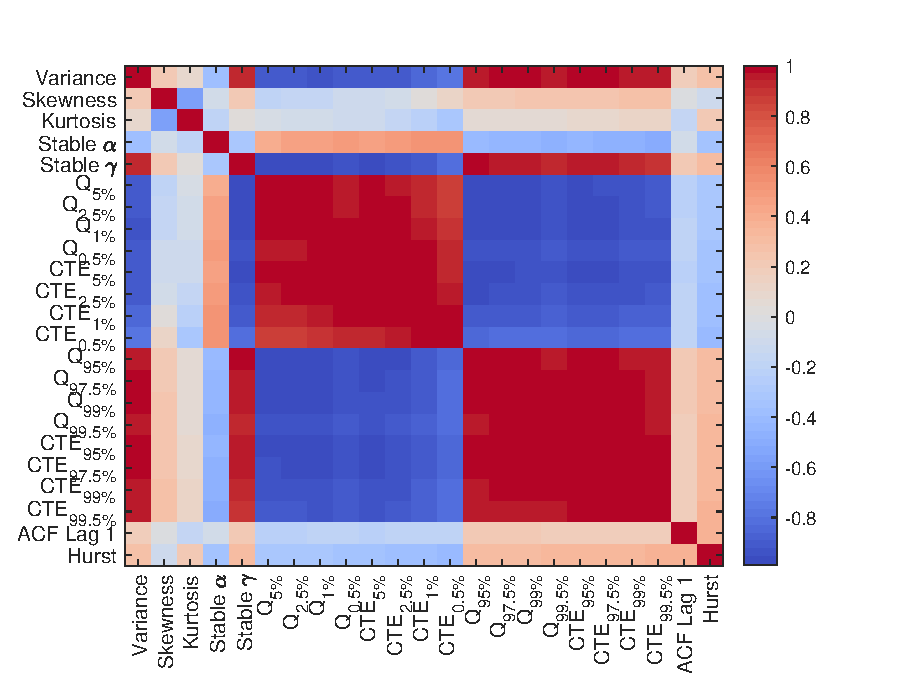
\includegraphics[width=1\textwidth]{Fig/figure_2}
      \caption{Correlation matrix\href{https://github.com/QuantLet/Genus_proximum_cryptos/tree/master/SFA_Cryptos}{. SFA\_cryptos}}
      \label{fig:figure_2}
  \end{minipage}
  \begin{minipage}[b]{0.53\textwidth}
\centering
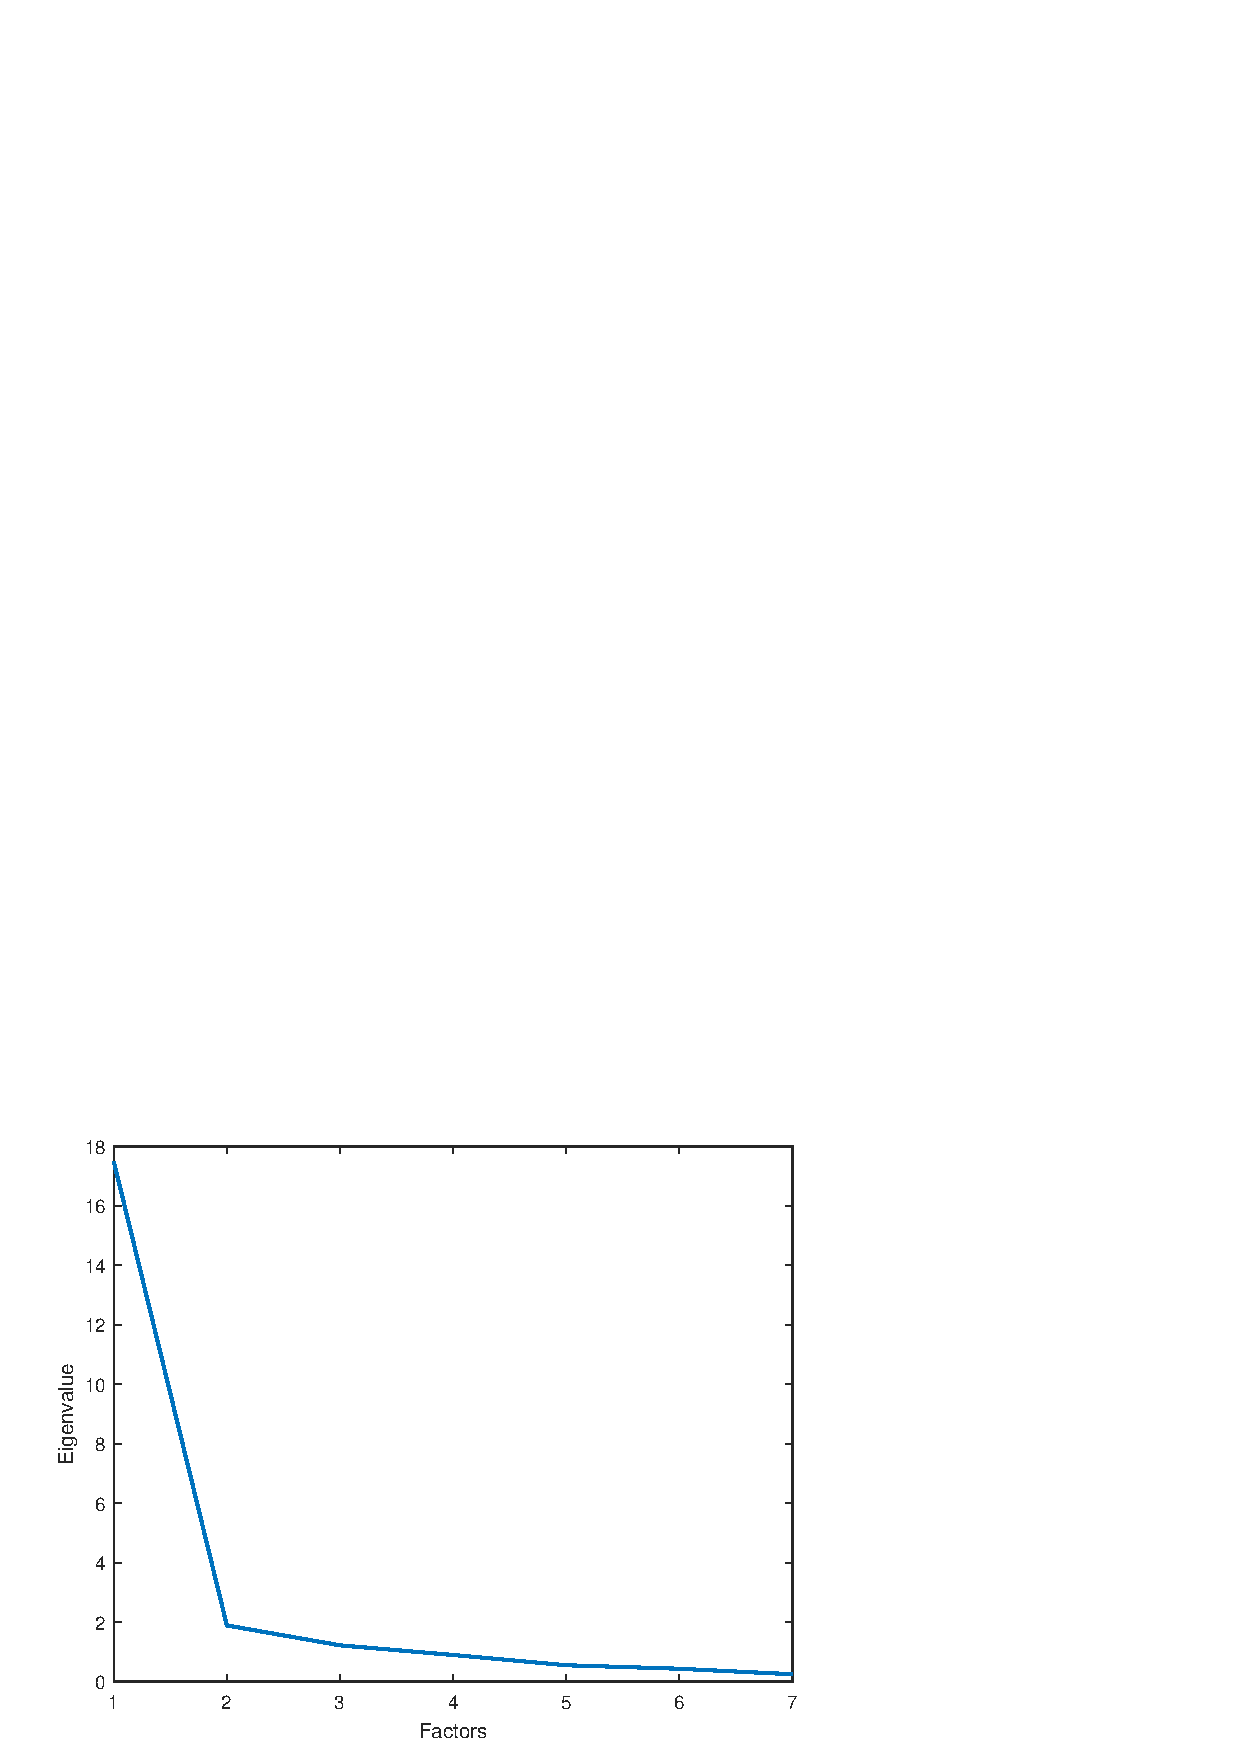
\includegraphics[width=1\textwidth]{Fig/figure_3}
  \caption{Scree plot\href{https://github.com/QuantLet/Genus_proximum_cryptos/tree/master/SFA_Cryptos}{. SFA\_cryptos}}
    \label{fig:figure_3}
  \end{minipage}
\end{figure}

Based on the eigenvalues criteria, we can select those factors for which the eigenvalue is higher than 1 (see the \hyperref[fig:figure_3]{Figure 3}, where the scree plot is shown). According to this criteria, three factors were selected, accounting for 89.6\% of the total variance.

In order to test the sampling adequacy of the factor analysis, we are using the Kaiser-Meyer-Olkin (KMO); the KMO test should be greater than 0.5 for a satisfactory factor analysis \citep{Tabachnick.op.2013}.\\
The overall KMO test is computed using the following formula:
\begin{align}
KMO=\frac{\sum_{i}\sum_{i\neq j}r_{ij}^2}{\sum_{i}\sum_{i\neq j}r_{ij}^2+\sum_{i}\sum_{i\neq j}u_{ij}^2}
\end{align}
where $R = r_{ij}$ is the correlation matrix and $U = u_{ij}$ is the partial covariance matrix \citep{Cerny.1977, Kaiser.1974}.\\
The individual KMO test is computed using the formula:
\begin{align}
KMO=\frac{\sum_{i\neq j}r_{ij}^2}{\sum_{i\neq j}r_{ij}^2+\sum_{i\neq j}u_{ij}^2}
\end{align}
In fact, the KMO measure represents the proportion of the variance in the input variables that might be caused by underlying factors \citep{Kaiser.1981}. The overall KMO value is $0.903$, pointing out that the factor analysis is suitable for structure detection (see \hyperref[table:table_3]{Table 3}). For the factor rotation, we used the VARIMAX method, which outputs orthogonal factors, also minimizing the number of variables that have high loadings on each factor.\\
\indent{}Based on the rotated factors pattern, the following conclusions can be drawn (see also \hyperref[fig:figure_4]{Figure 4}):
\begin{enumerate}
	\item The first factor – \textbf{the tail factor}, accounting for 76.1\% of the total variance, is highly correlated with the following parameters: the tail parameter alpha and the scale parameter gamma of the stable distribution, the lower and upper quantiles of the distribution of log-returns, the conditional tail expectations and the variance of log-returns.
	\item The second factor – \textbf{the moment factor}, accounting for 8.2\% of the total variance, is highly correlated with the skewness and kurtosis of the distribution of log-returns.
	\item The third factor – \textbf{the memory factor}, accounting for 5.3\% of the total variance, is highly correlated with the Hurst exponent and the first order autocorrelation coefficient of log-returns.
\end{enumerate}

\begin{table}[H]
\centering
\caption{: Kaiser's Measure of Sampling Adequacy}
   \label{table:table_3}
\small{
\begin{tabular}{llll} \hline \hline
Variable & KMO measure & Variable    & KMO measure \\ \hline
$Variance$         & 0.970       &  $Q_{99.5\%}$           & 0.893       \\
$Skewness$         & 0.540       &  $CTE_{0.5\%}$          & 0.877       \\
$Kurtosis$         & 0.510       &   $CTE_{1\%}$          & 0.892       \\
$Stable_\alpha$        & 0.935       &   $CTE_{2.5\%}$          & 0.928       \\
$Stable_\gamma$           & 0.861       &  $CTE_{5\%}$           & 0.884       \\
$Q_{0.5\%}$         & 0.923       &    $CTE_{95\%}$         & 0.878       \\
$Q_{1\%}$         & 0.932       &      $CTE_{97.5\%}$       & 0.898       \\
$Q_{2.5\%}$         & 0.921       &    $CTE_{99\%}$         & 0.884       \\
$Q_{5\%}$         & 0.915       &      $CTE_{99.5\%}$       & 0.874       \\
$Q_{95.5\%}$         & 0.899       &     ${\rho}(1)$        & 0.713       \\
$Q_{97.5\%}$         & 0.948       &     ${H}$        & 0.862       \\
$Q_{99\%}$         & 0.925       & Overall KMO & 0.903       \\ \hline\hline
\end{tabular}}

\end{table}




\begin{figure}[H]
\centering
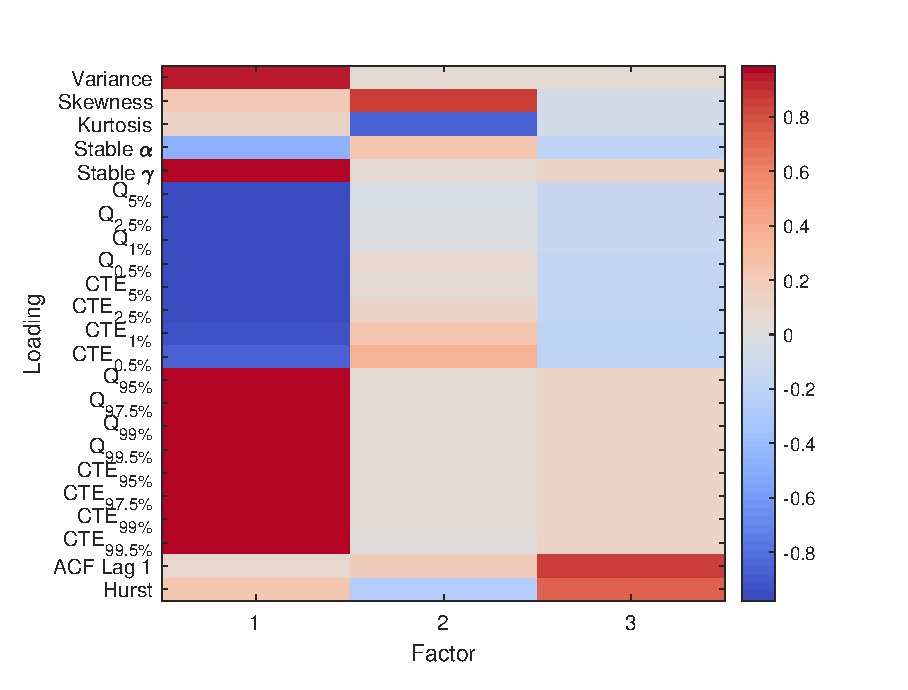
\includegraphics[width=0.65\textwidth]{Fig/figure_4}
\caption{Loadings of the three factors\href{https://github.com/QuantLet/Genus_proximum_cryptos/tree/master/SFA_Cryptos}{. SFA\_cryptos.}}
   \label{fig:figure_4}
\end{figure}

Based on the factors estimated through the factor analysis, one can map the cryptocurrencies and the classical assets, in order to derive some clustering effect.

\begin{figure}[H]
	\begin{minipage}[b]{0.55\textwidth}
		\centering
		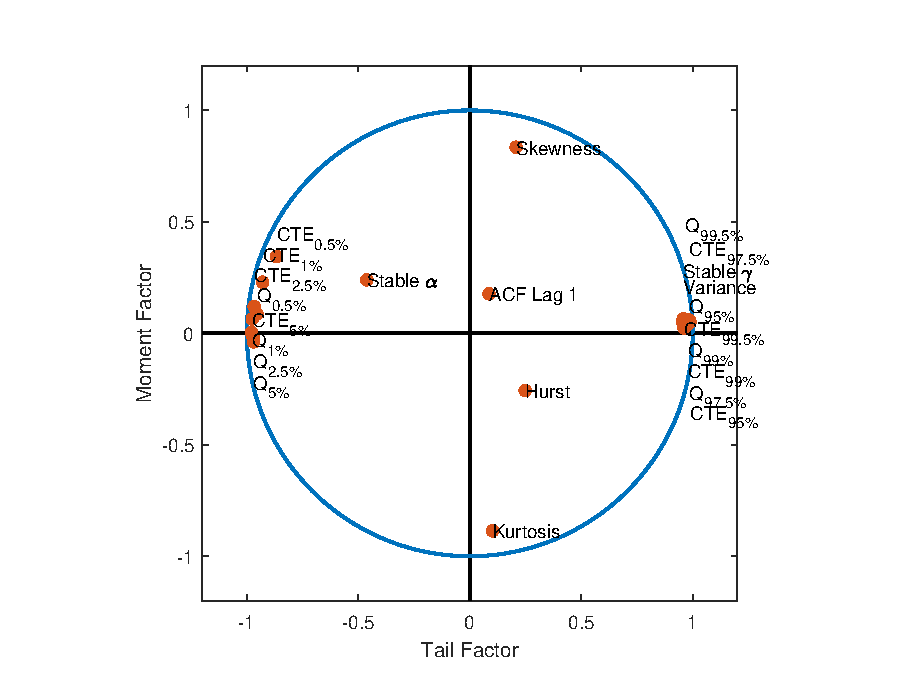
\includegraphics[width=1\textwidth]{Fig/figure_5a}


	\end{minipage}
	\begin{minipage}[b]{0.55\textwidth}
		\centering
		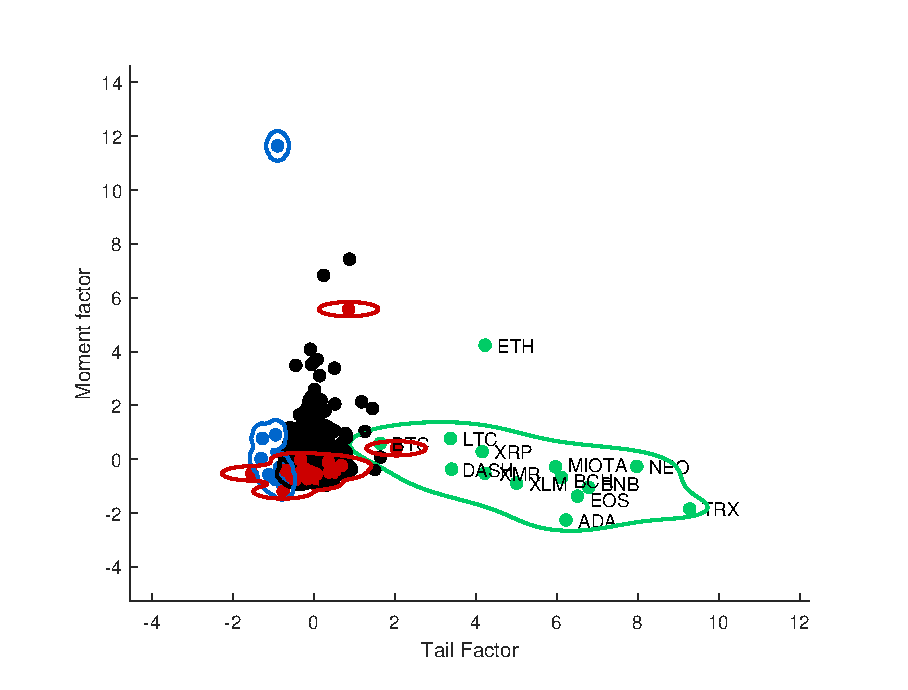
\includegraphics[width=1\textwidth]{Fig/figure_5b}

	\end{minipage}
\caption {Loadings (left) and scores (right) based on tail and moment factor\href{https://github.com/QuantLet/Genus_proximum_cryptos/tree/master/SFA_Cryptos}{. SFA\_cryptos.}}
\label{fig:figure_5}
\end{figure}



Figures 5 to 7 map the cryptocurrencies and the classical assets; the colour code is the following: green - cryptocurrencies, black – stocks, red – commodities, blue – exchange rates. Also, a $95\%$ confidence region is estimated, based on the Bivariate Kernel Density. 
\begin{figure}[H]
	\begin{minipage}[b]{0.55\textwidth}
		\centering
		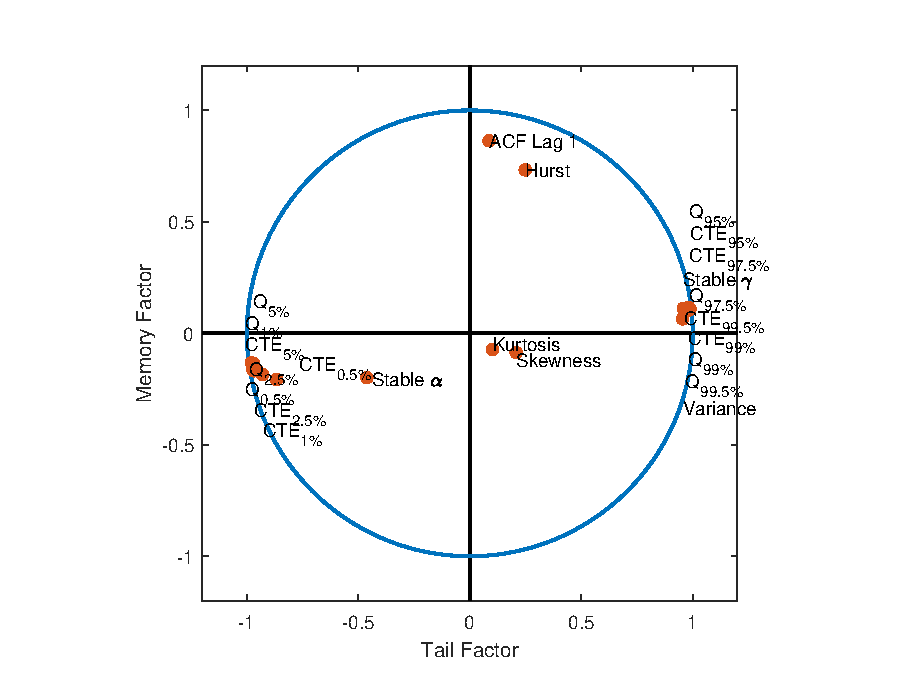
\includegraphics[width=1\textwidth]{Fig/figure_6a}
		
		
	\end{minipage}
	\begin{minipage}[b]{0.55\textwidth}
		\centering
		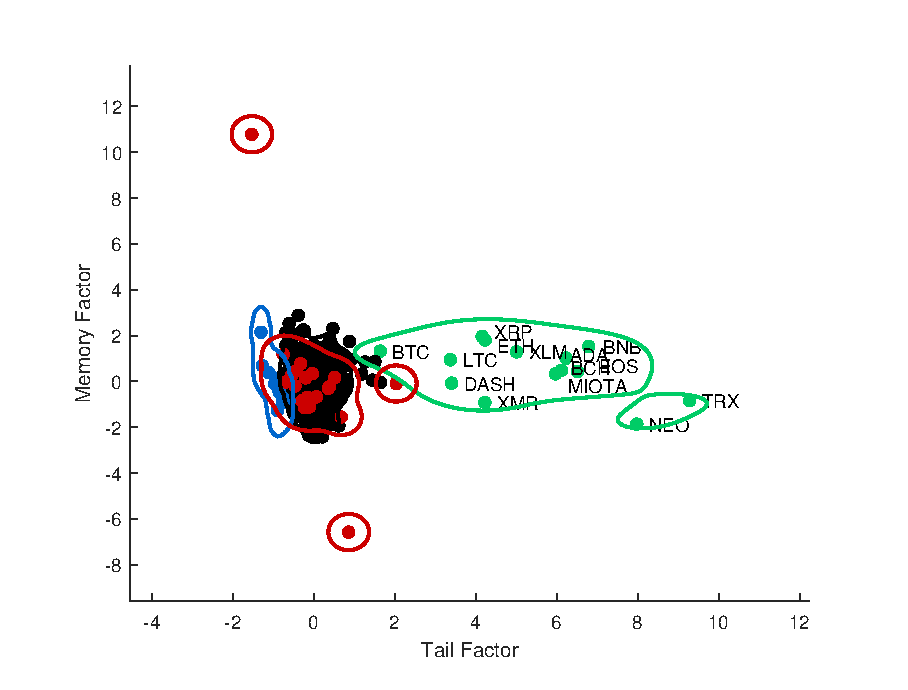
\includegraphics[width=1\textwidth]{Fig/figure_6b}
		
	\end{minipage}
	\caption {Loadings (left) and scores (right) based on tail and memory factor\href{https://github.com/QuantLet/Genus_proximum_cryptos/tree/master/SFA_Cryptos}{. SFA\_cryptos.}}
	\label{fig:figure_6}
\end{figure}

As shown in \hyperref[fig:figure_5]{Figure 5} and \hyperref[fig:figure_6]{Figure 6}, there is a clear separation between cryptocurrencies and classical assets, mainly due to the first factor, the tail factor, while the memory and moment factor are of subliminal subliminal importance (see \hyperref[fig:figure_7]{Figure 7}).
\begin{figure}[H]
	\begin{minipage}[b]{0.55\textwidth}
		\centering
		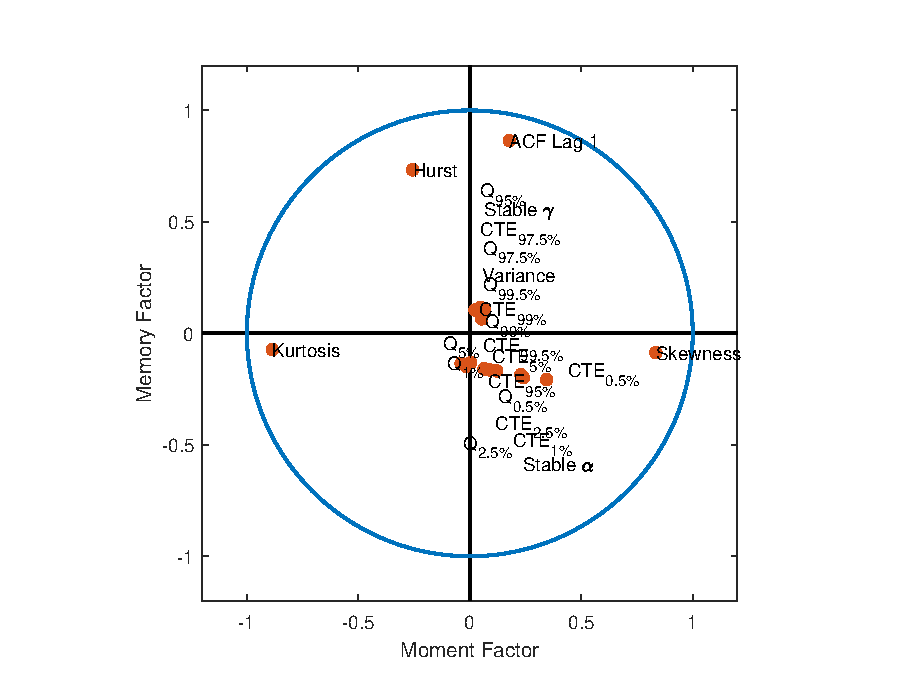
\includegraphics[width=1\textwidth]{Fig/figure_7a}
		
		
	\end{minipage}
	\begin{minipage}[b]{0.55\textwidth}
		\centering
		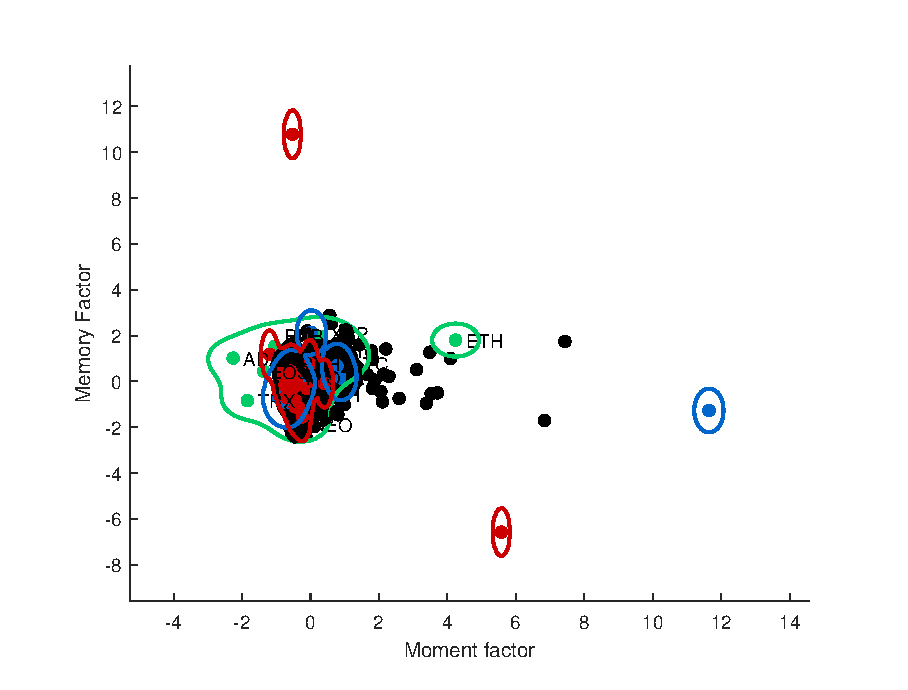
\includegraphics[width=1\textwidth]{Fig/figure_7b}
		
	\end{minipage}
	\caption {Loadings (left) and scores (right) based on moment and memory factor\href{https://github.com/QuantLet/Genus_proximum_cryptos/tree/master/SFA_Cryptos}{. SFA\_cryptos.}}
	\label{fig:figure_7}
\end{figure}

\indent{}Based on the data revealed in the \hyperref[table:table_4]{Table 4}, one can synthesize few characteristics of the cryptocurrencies, that differentiate them from the other assets:
\begin{itemize}
	\item The cryptocurrencies have higher variance of the log-return’s distribution, compared to the classical assets.
	\item The cryptocurrencies exhibit the presence of heavy tails, as indicated by high values of quantiles and conditional tail expectations, i.e. the cryptocurrencies have higher propensity for risk.
	\item The first order autocorrelation is positive in the case of cryptocurrencies, while all the other assets have negative first order autocorrelation, for the analysed time period.
	\item Bitcoin is closer to classical stocks and commodities, in terms of the tail factor, i.e. it’s risk profile can be considered at the border between the classical assets and cryptocurrencies.
\end{itemize}
\begin{table}[H]
	\centering
		\caption{: Assets profile based on the average values of the initial variables}
	\label{table:table_4}
	\small{
		\begin{tabular}{l|l    S[table-format=3.2, round-mode=places,round-precision=3] S[table-format=3.2, round-mode=places,round-precision=3] S[table-format=3.2, round-mode=places,round-precision=3] S[table-format=3.2, round-mode=places,round-precision=3] S[table-format=3.2, round-mode=places,round-precision=3] S[table-format=3.2,round-mode=places,round-precision=3] S[table-format=3.2, round-mode=places,round-precision=3] }\hline\hline
			\multicolumn{1}{l}{\bfseries Factor }&\multicolumn{1}{l}{\bfseries Estimate} &\multicolumn{1}{l}{\bfseries Cryptos}&\multicolumn{1}{l}{\bfseries Stocks} &\multicolumn{1}{l}{\bfseries Commodities} &\multicolumn{1}{l}{\bfseries Exchange Rates}  &\multicolumn{1}{l}{\bfseries Bitcoin}\\ \hline
			
			Tail        & $\sigma^2\cdot10^{3}$                 & 7.88  & 0.28      & 0.37         & 0.03 & 1.50  \\
			factor                 &   $Stable_\alpha$               & 1.436  & 1.703       & 1.753          & 1.759   & 1.319  \\
			&   $Stable_\gamma\cdot10^{3}$          & 36.76  & 8.73       & 9.85           & 3.17   & 16.02  \\
			&   $Q_{0.5\%}$               & -0.255 & -0.056      & -0.052         & -0.015  & -0.139 \\
			&   $Q_{1\%}$               & -0.215 & -0.044      & -0.043         & -0.013  & -0.113 \\
			&   $Q_{2.5\%}$               & -0.148 & -0.032      & -0.034         & -0.01   & -0.086 \\
			&   $Q_{5\%}$               & -0.113 & -0.024      & -0.026         & -0.008  & -0.063 \\
			&   $Q_{95\%}$               & 0.133  & 0.024       & 0.027          & 0.008   & 0.059  \\
			&   $Q_{97.5\%}$               & 0.198  & 0.03        & 0.035          & 0.01    & 0.082  \\
			&   $Q_{99\%}$               & 0.285  & 0.04        & 0.045          & 0.013   & 0.109  \\
			&   $Q_{99.5\%}$               & 0.383  & 0.05        & 0.056          & 0.015   & 0.139  \\
			&   $CTE_{0.5\%}$               & -0.326 & -0.077      & -0.072         & -0.022  & -0.184 \\
			&   $CTE_{1\%}$               & -0.278 & -0.063      & -0.06          & -0.018  & -0.152 \\
			&   $CTE_{2.5\%}$               & -0.217 & -0.048      & -0.046         & -0.014  & -0.123 \\
			&   $CTE_{5\%}$               & -0.172 & -0.038      & -0.038         & -0.011  & -0.098 \\
			&   $CTE_{95\%}$               & 0.233  & 0.035       & 0.04           & 0.011   & 0.092  \\
			&   $CTE_{97.5\%}$               & 0.307  & 0.043       & 0.049          & 0.013   & 0.116  \\
			&   $CTE_{99\%}$               & 0.411  & 0.055       & 0.065          & 0.016   & 0.147  \\
			&   $CTE_{99.5\%}$               & 0.499  & 0.067       & 0.08           & 0.019   & 0.175  \\
			Moment  &     $Skewness$             & 0.973  & -0.508      & 0.285          & -1.223  & -0.283 \\
			factor                 &   $Kurtosis$               & 20.351 & 12.922      & 20.716         & 33.992  & 8.583  \\
			Memory  &     $\rho(1)\cdot10^{3}$             & 40.63  & -2.16      & -13.18         & -11.45  & 16.64  \\
			factor                &    $H$              & 0.567  & 0.509       & 0.533          & 0.514   & 0.565  \\
			
			\hline \hline
	\end{tabular}}

\end{table}




\subsection{Assets classification}

In this section, we list the results of the models presented in Section 2.3, in order to assess the ability of the factors produced through the factor analysis to discriminate between cryptocurrencies and classical assets.\\
First, for each of the three factors we estimated the binary logistic model:
\begin{align} \label{form:logit_est}
P(Y_{i}=1)=\frac{\exp(\beta_{0 j}+\beta_{1 j} F_{j i})}{1+\exp(\beta_{0 k}+\beta_{1 j} F_{j i})},
\end{align}

where $Y_{i}=1$ for cryptocurrencies, $Y_{i}=0$ for classical assets, and $F_j, j\in\left\{1,2,3\right\}$ are the $3$ orthogonal factors retrieved through the factor analysis.

\hyperref[table:table_5]{Table 5} lists the estimated $\beta_{1 j}$ of the binary logistic regression model \ref{form:logit_est}, with the performance measure defined by the equation \ref{form:pseudoR}.

\begin{table}[!ht]
\centering
\small{
\caption{: Estimates of the model \ref{form:logit_est}}
\label{table:table_5}
\begin{tabular}{p{1.5in} p{0.7in} p{0.7in} p{0.7in} } \hline \hline
	\textbf{Exogenous factor} & \textbf{Factor 1} & \textbf{Factor 2} & \textbf{Factor 3} \\ \hline 
	Esimated $\beta_{1}$ & 4.398** & -3.729 & -3.692 \\  
	& (2.086) & (-0.606) & (0.314) \\
	\textit{pseudo-}$R_{adj}^{2} $ & 0.958 & 0.015 & 0.024 \\  
	\hline \hline
\end{tabular}
\\Note: Standard errors in (); ** denotes significance at 95\% confidence level.
\noindent }
\end{table}

As seen in \hyperref[table:table_5]{Table 5}, the most important factor regarding the separation between the cryptocurrencies and the classical assets is the tail factor, while the other two factors have no significant influence.\\
Second, we employed Discriminant Analysis and Support Vector Machines on the space defined by the two first factors (tail and memory).
\hyperref[fig:figure_8]{Figure 8} presents the classification results using Discriminant Analysis. Both linear and quadratic classifiers have a very good classification power, the only cryptocurrency which is misclassified being the Bitcoin (see the \hyperref[table:table_4]{Table 4} for Bitcoin's profile).


\begin{figure}[!ht]
\begin{minipage}[b]{0.48\textwidth}

\centering
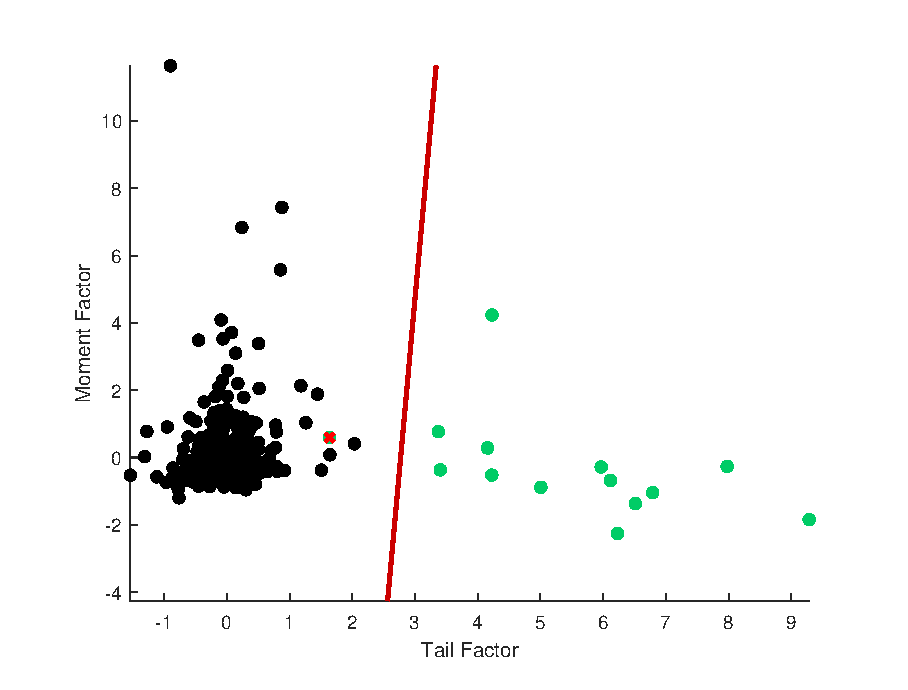
\includegraphics[width=1\textwidth]{Fig/figure_8a}


\end{minipage}
\begin{minipage}[b]{0.48\textwidth}

\centering
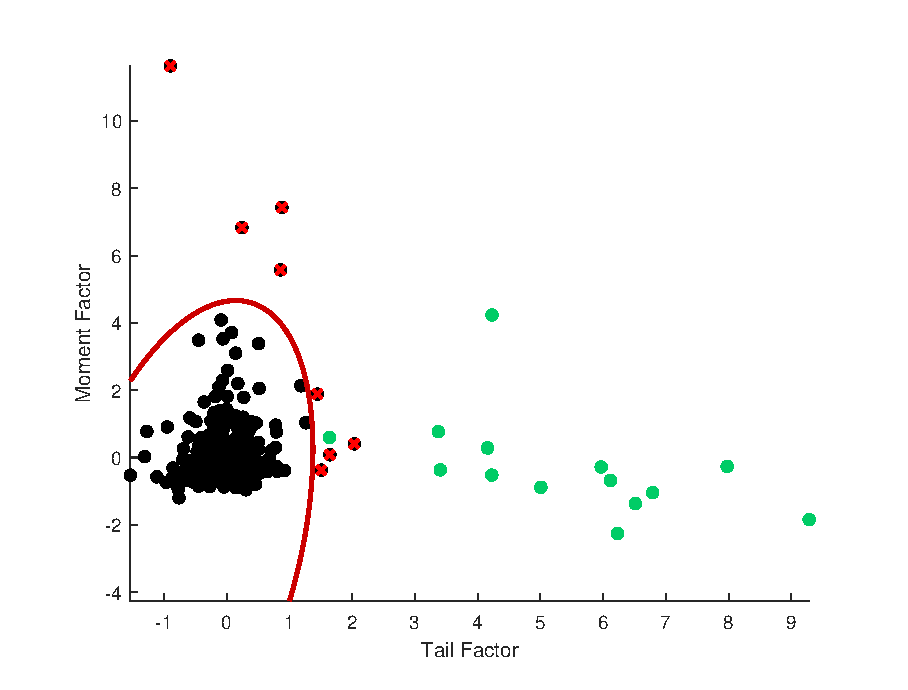
\includegraphics[width=1\textwidth]{Fig/figure_8b}


\end{minipage}
\caption{ Discriminant Analysis: linear(left) and quadratic (right). Green dots denote the cryptocurrencies, while the black dots denote the other assets; the dots highlighted in red are cases of misclassification\href{https://github.com/QuantLet/Genus_proximum_cryptos/tree/master/SFA_Cryptos}{. SFA\_cryptos.}}
	\label{fig:figure_8}
\end{figure}

The same conclusion can be drawn by looking at the results of the Support Vector Machines non-linear classifier, according to which all the cryptocurrencies are correctly classified using the tail factor and the moment factor (see \hyperref[fig:figure_9]{Figure 9}).

\begin{figure}[!ht]
\centering
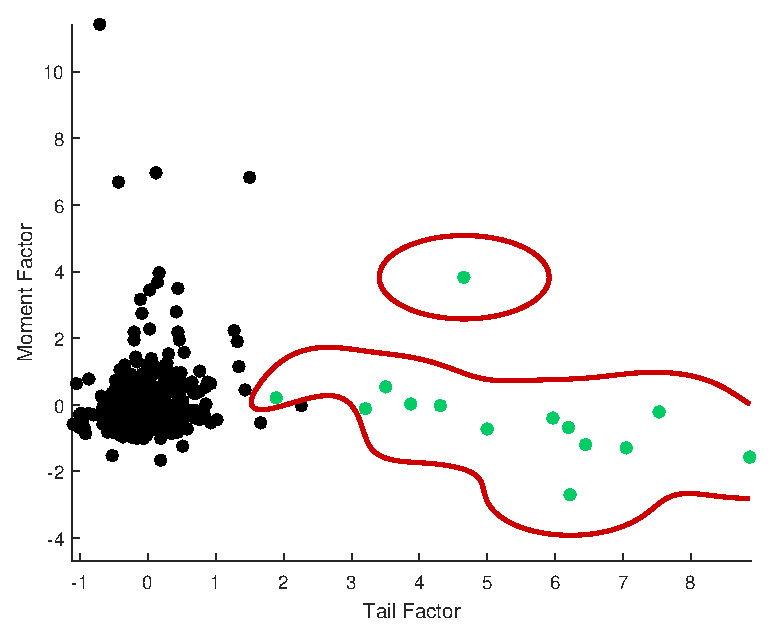
\includegraphics[width=0.48\textwidth]{Fig/figure_9}
\caption{ Support Vector Machines. Green dots denote the cryptocurrencies, while the black dots denote the other assets\href{https://github.com/QuantLet/Genus_proximum_cryptos/tree/master/SFA_Cryptos}{. SFA\_cryptos.}}
	\label{fig:figure_9}
\end{figure}

From an Aristotelian point of view, we can conclude that the differentia specifica of the cryptocurrencies is the tail behaviour of the distribution of daily log-returns.
In other words, based on the tail factor profile, we can conclude that a random asset is likely to be a cryptocurrency if it has the following properties: very long tails of the log-returns distribution (in terms of the left and right quantile and the conditional tail expectation), high variance, high value of the alpha stable scale parameter and value of the alpha stable tail index closer to 1.


